\documentclass{article}
\usepackage[utf8]{inputenc}
\usepackage{multirow}
\usepackage{verbatim}
\usepackage[pdftex]{graphicx}
\usepackage{subfigure}


\begin{document}
\title{\textbf{Profiling users media preferences based on social network data streams}}
\author{Konrad Delong \and Antoni Piechnik}
\date{June 27 2010}

\maketitle

\begin{abstract} Social networks have been becoming hugely popular over the last
years. With enormous number of people sharing information about their lives,
they are now a great source of information about their media interests. Based on both
structured data (such as the social aspect of \textit{YouTube}\footnote[1]{http://www.youtube.com}) as well as unstructured
(\textit{Twitter}\footnote[2]{http://www.twitter.com}), we analyze what data can be extracted from their profiles as well as
how useful such extraction is for profiling those users. Such profiling could
prove hugely influential for media-oriented recommender systems, such as the one
used in the \textit{NoTube}\footnote[3]{http://www.notube.tv} project.
We focus on aggregating and analyzing the publicly available data and covering
different approaches of profile generation
for users. Our experiments reveal multiple ways of employing social networks'
data for users profiling as well as show promising results for possibly employing
this data in a real-life project.
\end{abstract}

\section{Introduction}

Recommender systems used to involve recommending more physical objects \cite{combining-cf-with-pa} to users.
However, more and more abstract topics are becoming parts of such recommenders (such as tags) \cite{accuracy-recommending}. The NoTube project bases its recommendation of TV programmes on aggregating,
extracting and analyzing user activities \cite{notube-main}. The Web provides traces left by users
of social services regarding their activities, varying from user video viewing history
and subscriptions to video channels (e.g. \textit{YouTube})
to users' activity updates formed in natural language (such as \textit{Twitter}) \cite{why-we-twitter}.

In this paper we analyze those data streams and evaluate their usefulness to the \textit{NoTube}
project, by answering two main research questions.

Firstly, we find out \textit{what user data we can collect from both structured and natural language-based social applications?}. We mainly focus on researching the available data and analyze the way people use services such as
\textit{YouTube} and \textit{Twitter} to share their media preferences (Section 3).

Furthermore, we look into \textit{how do those services compare when it comes to automated user media
preference profile generating?}. In this part of the paper we present methods of evaluating results of
the aggregation of available data (Section 5) as well as actual user preferences profiling for both
services with a comparative analysis and discussion of the latter (Sections 6 and 7). Our research reveals that despite the
differences between those streams, both of them may provide enough opportunities for user media preference
extraction. We conclude with a summary (Section 8) followed by an overview of the particular implementation methods (Section 9).

\section{Related work}

A considerable number of papers examining social Web services have been
published. Works devoted to YouTube often contain analysis of the video data
stored by the service and its implications to the traffic generated
(\cite{i-tube-you-tube}, \cite{views-from-the-edge},
\cite{statistics-and-social-network}), some study impact of YouTube service on
very narrow topics, like 2006 USA presidential elections
\cite{voters-myspace-youtube}, or social attitude towards vaccinacions
\cite{keelan}. There are also papers analyzing privacy issues of using YouTube
\cite{publicly-private}.

Works analyzing \textit{Twitter} as a data stream can differ from very general \cite{why-we-twitter},
to works devoted to analyzing content of the \textit{Twitter} users' timelines (such as \cite{twitter-content-is-it} and \cite{short-tweet}).

There are also works devoted to automated user profile generation, covering multiple data sources for profile
information aggregation \cite{public-profiles}, as well as abusing social networks for profile generation \cite{twitter-abuse}. Apart from profile generation, a URL recommender system for \textit{Twitter} users
has been introduced by \cite{short-tweet}.

Apart from the papers mentioned, we have also found various implementations of systems that aggregate personal preferences based on different
social services:

\paragraph{Hunch}
\textit{Hunch}\footnote[2]{http://www.hunch.com}) is a service offering recommendations on different topics based on a user's \textit{Twitter} data. It predicts preferences in forms of small questions and is then able to recommend a product or a solution to a problem that is represented with a \textit{Topic} on the site. \textit{Hunch} seems to be more commercial-oriented, e.g. providing users with links to online stores with products they are recommending. However,
it's prediction results suggest that \textit{Twitter} users' timelines contain information about their preferences.

The application can create recommendations based solely on user's \textit{Twitter} data (mostly people they follow). However, when little is available, it requires input from users in order to make future predictions more accurate. It covers topics broader than the \textit{NoTube} project.
\textit{Hunch.com} does not provide information on how the recommender system works, although it provides an API for accessing their data.
Hunch is able to adapt to much more different topics, and it not necessarily focuses on their semantics (rather on what similar people simply like).

\section{User activity data on the Social Web} 
\label{sec:uad}
In order to answer the first research question, we have focused on data from two social services: \textit{YouTube} and
\textit{Twitter}. The goal of this chapter is to present the organization of the \textit{user activity data} (UAD)
available in those two networks.

In the section \ref{sec:youtube_uad} we describe user data available via APIs for
\textit{YouTube}, whereas section \ref{sec:twitter_uad} covers possible methods of extracting preference information
from \textit{Twitter} users' tweets. We will use the expression \textit{named entity} (NE) to refer to
known media people, shows and programs. The NE data has been collected from the \textit{Freebase} dataset,
which we described in section \ref{sec:vocabulary}.

\subsection{YouTube}
\label{sec:youtube_uad}

\textit{YouTube} stores various data concerning its users and content and offers a public
access to this structured information through the use of its API. In theory, additional
pieces of data could be acquired through the use of screen scraping. Using this
technique, however, breaks \textit{YouTube}'s Terms and Conditions (\S 5.1H), and as such
was not used for this research.

The schema of \textit{YouTube} data is presented in tables 1-5.  Each table lists
properties of a single type of entity, along with the way those properties are
accessed (either API or through the use of screen scraping). For example:
we can learn that values of such video's parameters as its view count or
its duration (and many others) are accessible through the official API.

Among these elements, what begs for most attention are the video sets.
Undoubtedly, videos are the central point of \textit{YouTube} as a service, and form the
majority of its content. This sets them as most suitable candidates for data
enrichment. Furthermore, the user can form a relation with a video by performing
an action on it (uploading, adding to favourites or subscribing), which makes
video analysis a perfect choice for semantic user profile generation.  Three
sets of videos are accessible through the official API, these are
\emph{favorites}, \emph{subscriptions} and \emph{uploads}. For this reason, the
rest of \textit{YouTube} research in this paper will focus on these three sets. The other
fields concerning user, like his \textit{age} or \textit{location}, while
directly usable as a part of the profile, are not as challenging to extract and
will not be analyzed in deep detail. \textit{YouTube} also contains demographic data
of a user, which we will not use in our experiments.

\begin{center}
  \begin{tabular}{|p{3cm} | l | p{4cm}|} \hline
  Information & Access & Notes\\ \hline
  Title & Public API & Natural language \\
  Published & Public API & \\
  Updated & Public API & Date \\
  Category & Public API & Chosen from a restricted set of YouTube categories \\
  Tags (keywords) & Public API & May be freely assigned \\
  Comments & Public API & Natural language \\
  Permissons & Public API & Irrelevant, but available \\
  Description & Public API & Natural language \\
  Thumbnails & Public API & Set of video's thumbnails (along with times
  when taken) \\
  Duration & Public API & \\
  Ratings & Public API & Best, worst and average rating, number of votes \\
  Viewcount & Public API & \\
  Favourite count & Public API & \\
  Number of likes & Public API & \\
  Number of dislikes & Public API & \\
  Aspect ratio & Public API & \\
  Related & Public API & \\
  Responses & Public API & \\
  Author & Public API & \\ \hline
  \end{tabular} \\
  Table 1: Information available for a video \\
\end{center}

\begin{table}[htb]
	\begin{minipage}[b]{0.5\linewidth}
	\centering
		\begin{tabular}{ | p{3cm} | l |}\hline
		Information & Access \\ \hline
		Number of results & Public API \\
		Search results & Public API \\ \hline
		\end{tabular}
		Table 2: Information available for video search results \\

		\begin{tabular}{ | p{3cm} | l |}\hline
			Information & Access \\ \hline
			Created & Public API \\
			Updated & Public API \\
			Author & Public API \\
			Text & Public API \\ \hline
		\end{tabular}
		Table 3: Information available for a comment \\

		\begin{tabular}{ | p{3cm} | l |}\hline
			Information & Access \\ \hline
			Demographics & Screen scraping \\
			Referrers & Screen scraping \\
			Countries popularity & Screen scraping \\ \hline
		\end{tabular}
		Table 4: Information available for a channel \\
	\end{minipage}
	\hspace{0.5cm} % no new lines here!!
	\begin{minipage}[b]{0.5\linewidth}
		\centering
		\begin{tabular}{ | p{3cm} | l |}\hline
			Information & Access\\ \hline
			\emph{Uploads} & Public API \\
			Gender & Public API \\
			Location & Public API \\
			Age & Public API \\
			Contacts & Public API \\
			Username & Public API \\
			\emph{Subscriptions} & Public API \\
			Inbox & Public API \\
			\emph{Favorites} & Public API \\
			History & Screen scraping \\
			Likes & Screen scraping \\
			Issued authentication subtokens & Screen scraping \\ \hline
		\end{tabular}
		Table 5: Information available for a user
		\label{ut_user_info}
	\end{minipage}
\end{table}

\subsubsection{Problems regarding concepts identification}

Even though the video sets are most promising mean to interest extraction. There
are problems that make this task challenging.

\paragraph{Detecting level of interest}
One of them, is the fact that YouTube videos cannot
express an interest directly. The user can add a video to the favourites
indicating some level of interest, but we are not able to detect the reason for
such user's action. This indirectness might result in lower precision of the
interests extracted from YouTube. 

The only indicator of an interest in a particular subject is binary: it is
either present or not present in user's data. This forces us to fall back to
entity counting in order to determine level of interest.

\paragraph{Usage of YouTube features} 
Another problem is the scarcity of data. Below are measurements that showed how
little users make extensive use of YouTube features.
In order to find out how frequently the mentioned sets are used, a sample of 7,500
randomly chosen users was examined. Among those users, noticeable differences in their
activity (level of use of various features) were noted. Many users show little activity,
as compared to a few highly active users.  50\% analyzed accounts had less than 60 favourites,
6000 out of 7,500 had less than 40 uploads.  All histograms on Figure 1 show
numbers of users (axis y) with $x_1-x_3$ numbers of
favourites/subscriptions/uploads. For all three cases, almost all users belonged
to the first histogram range -- the one with least items. As number of items
grows, the number of users decreases so quickly, that logarithmic scale has been
used in order to increase the readability of the charts.

For all three sets, almost half of examined users had no more than 100 items.
This means that for most cases, the user profiling would need to be based on
little amount of data.

\begin{figure}[htb]
  \centering
  \subfigure[Favourites]{
		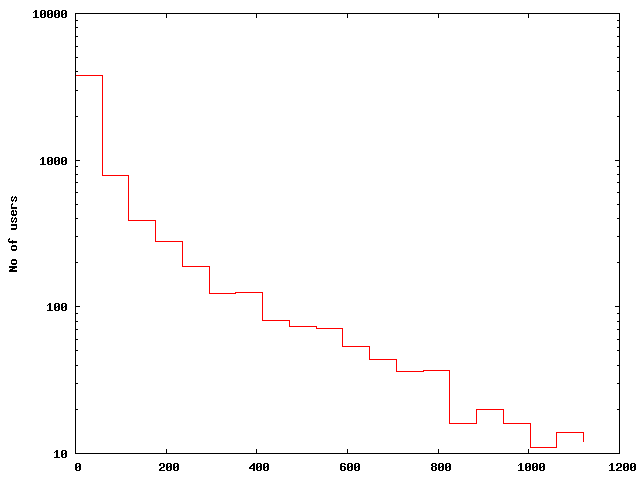
\includegraphics[scale=0.6]{images/favs.png}
		\label{fig:favs}
  }
  \subfigure[Subscriptions]{
		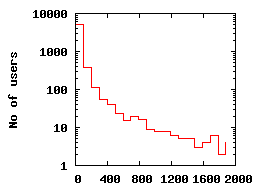
\includegraphics[scale=0.6]{images/subs.png}
		\label{fig:subs}
  }
  \subfigure[Uploads]{
		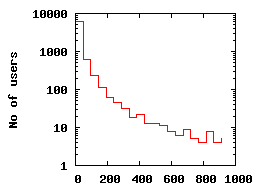
\includegraphics[scale=0.6]{images/ups.png}
		\label{fig:ups}
  }
  \label{fig:subfigureExample}
  \caption{Histograms of usage of favourites \subref{fig:favs}, subscriptions
  \subref{fig:subs} and uploads \subref{fig:ups}. The x axis represents groups of
  users having $x_1-x_2$ entities, the height of the bars indicates sizes of the
  groups.}
\end{figure}

\subsubsection{YouTube measurements employed}

We have decided to measure the user data in two ways: by identifying entities
and collecting tags. Each YouTube video contains a set of tags - single,
separate words - describing the video's content. While this kind of information
is not directly usable for the recommender systems, it can prove indirect
support for verifying the hypothesis that recommenders prepared. The types of
measurements performed are presented in Table 6.

\begin{center}
  \begin{tabular}{ | p{4cm} | p{7cm} | } \hline
    \multicolumn{2}{|c|}{Types of measurements available} \\
    \hline
    \multirow{3}{*} {Tag collection}
      & Tags from favourites \\ \cline{2-2}
      & Tags from subscriptions \\ \cline{2-2}
      & Tags from uploads \\ \cline{2-2}
    \hline
    \multirow{3}{*}{Concepts detection}
      & Concepts from favourites \\ \cline{2-2}
      & Concepts from subscriptions \\ \cline{2-2}
      & Concepts from uploads \\ \cline{2-2}
    \hline
  \end{tabular}
Table 6: Overview of the measures available for the \textit{YouTube} structured data \\
\end{center}

\subsubsection{YouTube video descriptions corpus}

A corpus of titles and descriptions for little over 100,000 videos was collected
for text-based analysis of YouTube data. The file's size was 36 Mbytes. This
data was used to compute number of video descriptions with identifiable concepts from
\textit{Freebase}\footnote{http://freebase.com} data vocabularies (more on this in section 4).

\subsection{Twitter}
\label{sec:twitter_uad}

Data available on \textit{Twitter} is composed of natural language short messages posted by users
consisting of up to 140 characters, commonly known as \textbf{tweets}. Within
those tweets we can distinguish user mentions (\textit{Twitter} usernames preceeded with the symbol @,
such as \textit{@justinbieber}\footnote{http://twitter.com/justinbieber}) as well as topics in form of
\textit{hashtags} -- names stripped of all whitespace and preceded by the hash symbol,
\eg \textit{\#TheDailyShow} \cite{edinburg-corpus}.

The initial purpose of tweets was to inform other users of currently performed activities. However, as this service has
evolved, users started to use \textit{tweets} for a variety of purposes, such as conversations,
sharing information/URLs and reporting news \cite{why-we-twitter, twitter-content-is-it}. In this section we describe available methods to use such unstructured data.
In our experiments we focus on the following NE extraction methods:

\paragraph{Mentioning NE full names}
Using simple string matching methods, we search for NE labels within tweets.
Occurrences of NE names in tweets indicate a potential interest in the NE mentioned. The
number of references is expected to be positively correlated with the level of interest in the given NE \cite{twitter-content-is-it}.
Entities might be mentioned by:
\begin{itemize}
  \item \textit{full name} (\eg \textit{"Having a How I Met Your Mother marathon."})
  \item \textit{hashtag} (\eg \textit{"Who?! Where? I love \#HowIMetYourMother!"})
  \item \textit{twitter username} (NE's twitter username, if known, \eg \textit{"@HIMYM\_CBS It entertains the spirit"})
  \item \textit{acronyms} (\eg \textit{"Watching HIMYM. Season 3."})
\end{itemize}
\paragraph{Usage of opinion vocabulary when tweeting about NEs}
In order to extract opinion towards a NE from a tweet, vocabularies that express
opinion has been compiled. They have been pragmatically chosen by looking at random tweets.
This vocabulary contains the following words: \textit{awesome, bad, enjoyed, good, great, hate,
like, liked, love, loving, poor, recommend, stunning, worst}.
Those verbs were searched for in the tweets containing NE mentions.
Example of a tweet: \textit{"yesterday's \#Lost episode was stunning!"}
\paragraph{Usage of activity verbs when tweeting about NEs}
When mentioning a media-related NE, users may also describe the activity performed.
In order to find such tweets, an activity verbs vocabulary has been prepared (similarly to
the opinion verbs, it was chosen by looking at the contents of random tweets).
This vocabulary contains the followings verbs: \textit{watching, watched, play,
watch, playing, saw, seen, played}.
Describing the activity of participating in a certain TV experience, such
as watching a show, has to be noted due to the fact that Twitter users are more
likely to specify what they are doing at a particular moment.
Example of a tweet: \textit{"Finnally watched Ironman 2 aha'"}

\paragraph{Extracting NEs from structured twitter stream sources}
Applications, such as \textit{YouTube} or \textit{Boxee}\footnote{http://www.boxee.tv}, automatically generate tweets
if the user linked their Twitter account with that application. These tweets are
usually well structured, and therefore very suitable to extract a NE, activity or preference.
Examples of tweets: (\textit{Boxee}) -- \textit{"likes Inglourious Basterds on Boxee http://bit.ly/FbAbn"} and
\textit{YouTube} -- \textit{"I liked a YouTube video -- How I Met Your Mother - Lorenzo Van Matterhorn"}

\paragraph{Summary}
We present the possible measurements for extracting the UAD from
\textit{Twitter} in Table 7:

\begin{center}
  \begin{tabular}{ | p{4cm} | p{7cm} | } \hline
    \multicolumn{2}{|c|}{Types of measurements available} \\
    \hline
    \multirow{4}{*} {Mentioning NEs}
      & Full name matching \\ \cline{2-2}
      & Matching the twitter username (if known) \\ \cline{2-2}
      & Matching name converted to a hashtag form \\ \cline{2-2}
      & Matching the full name acronym \\ \cline{2-2}
    \hline
    Usage of activity verbs & Mentions using activity verbs \\
    \hline
    \multirow{3}{*}{Using preference verbs}
      & Mentions using preference verbs \\ \cline{2-2}
      & Positive preferences \\ \cline{2-2}
      & Negative preferences \\ \cline{2-2}
    \hline
  \end{tabular}
Table 7: Overview of the measures available for the \textit{Twitter} UAD extraction \\
\end{center}

\subsubsection{Corpus used for research}

The example data analyzed consists of 43,000 tweets of 203 different users.
They have been selected by looking at the followers of popular TV channels and broadcasters
available on Twitter. Users were selected based on the number of tweets and their followers.
For our experiments, we have focused on tweets in English.

The most significant reason for using a precompiled corpus for this research is the Twitter API
Rate Limiting which limits the amount of tweets that can be fetched using the API.
Furthermore, a great deal of Twitter users provide data not necessarily
useful for our experiments. Mentions of NEs in non-English tweets could be located, but
extracting preference information in a multi-lingual setting is more challenging.
Using a preselected corpus enables measuring and comparing the effectiveness of different
counting methods much easier \cite{short-tweet}.

\subsection{Metrics used in constructing User Profile}

The generated user profile is a collection of concepts along with their
weights. In order to keep the scale of the weight simple (more on that in section
\ref{sec:evaluation}), we limited the scale to an integer range from 0
up to 3, meaning accordingly: ''do not like'', ''neutral'', ''like'', ''like
very much''. In order to determine the weight for each concepts, simple metrics
were used: number of repeats normalized to the mostly repeated item for
YouTube, and type of mention, the amount of mentions of a specified NE as well
activity/preference vocabulary usage for Twitter.



\section{Vocabulary}

\paragraph{Dataset used}
In order to link the concepts in the user profile to known uniquely identifiable concepts in the Linked Open Data
cloud\footnote{http://linkeddata.org}, we used vocabularies from the \textit{Freebase} service.

Freebase is a service offering a large (over 10 million topics) amount of semantically linked data on various topics.

The data available on Freebase is divided into \textit{topics}, types and properties. \textit{Topics} correspond to data
freely available, similar to \textit{Wikipedia}, describing physical entities, artistic creations, abstract concepts
etc. In comparison to \textit{Wikipedia}, all of the data on \textit{Freebase} is semantically structured,
allowing users to edit, add and remove data. As mentioned, the \textit{Freebase} project is a part of Linked Open Data.

\textit{Types} refer to different aspects of the same topic (\eg \textit{Bob Dylan} is a song writer,
singer and a film actor which all represent different types). All types have properties referring those
types to the topics (such as songs that Bob Dylan has written).

All topics and types have IDs expandable into URIs pointing to their location in the \textit{Freebase} dataset
(such as \textit{/en/tina\_fey}\footnote{www.freebase.com/view/en/tina\_fey} for actress \textit{Tina Fey}
or \textit{/medicine/disease}\footnote{www.freebase.com/view/medicine/disease} for the type \textit{Disease}).
By referring to those IDs a user is able to search Freebase for more linked data regarding the interesting topic and type.

From the whole wealth of data, we have focused only on the data related to the media, such as TV Actors, Movies, Movie
actors and TV Programmes as well as Bands and Singers' names.

\paragraph{Usage in the research}
We have decided to use the \textit{Freebase} dataset in order to be able to uniquely identify mentions of different NEs
within the available UAD. This approach is beneficial for use with recommender systems (such as the recommender
in the \textit{NoTube} profject), enabling them to immediately use the wealth of relational semantic data available
in the \textit{Linked Open Data cloud} for expanding their recommendations to related concepts.


\section{Using structured user activity data from YouTube}

Our goal is to extract a user profile. For this paper, we will assume that user
profile is a collection of linked data concepts and weights, that should be understood as
user's interests. Many YouTube videos have semantic meaning -- they can
be associated with existing concepts (like actors or music bands) by performing
text search. In addition to that, analysis of tags can give an overview of user's
interests. This kind of data is useful in two
ways: first, it lets easily identify interests for a user, second: it can be
used to verify interests generated with other methods..

In the following sections, we will describe methods used to generate the user
profile. First, we describe our tag counting approach and compare the possible
use of tags and categories in user profiling. Then we will discuss possible
additional information coming from repeating occurrences of the tags in
different sets of videos. The next subsection present the double
nestedness problem, which makes counting tags from subscriptions fundamentally
different that the other two sets. The last subsection describes matching
YouTube videos to actual linked data concepts.

\subsection{Counting YouTube tags and categories}
Analyzing tags information carries some problems. Tags of a single video clip
can be either too numerous, making many
of them irrelevant, too sparse, nonexistent and occasionally just wrong. To avoid
that problem, we aggregate the tags across sets of video clips related to the
profiled user (favourites, subscriptions, uploads). Similar aggregation was
performed for the videos' categories. Below is a comparison of results of counting
tags (chosen by the user) and categories (picked from a small predefined set).


\begin{table}[ht]
\begin{minipage}[b]{0.5\linewidth}\centering

\begin{tabular}{| l | l |}
Category & \# \\ \hline
News & 8 \\
Music & 5 \\
Education & 3 \\
Comedy & 2 \\
\end{tabular}

\end{minipage}
\hspace{0.5cm}
\begin{minipage}[b]{0.5\linewidth}
\centering

\begin{tabular}{| l | l |}
Tag & \# \\ \hline
sonik & 5 \\
bogusław & 5 \\
trzech & 5 \\
kupli & 5 \\
wybory & 4 \\
kraków & 4 \\
polska & 4 \\
\end{tabular}

\end{minipage}

\caption{Most popular tags and categories from account of Bogusław Sonik -- a
polish politician. The word ''wybory'' stands for ''election'' in polish, and
\emph{Trzech kumpli} is a title of a controversial political documentary.}
\end{table}


\begin{table}[ht]
\begin{minipage}[b]{0.5\linewidth}\centering

\begin{tabular}{| l | l |}
Category & \# \\ \hline
Music & 53 \\
Comedy & 20 \\
Entertainment & 8 \\
Games & 4 \\
People & 3 \\
Travel & 3 \\
News & 2 \\
\end{tabular}

\end{minipage}
\hspace{0.5cm}
\begin{minipage}[b]{0.5\linewidth}
\centering

\begin{tabular}{| l | l |}
Tag & \# \\ \hline
metal & 17 \\
music & 11 \\
rock & 11 \\
video & 7 \\
the & 7 \\
black & 7 \\
of & 7 \\
\end{tabular}

\end{minipage}

\caption{Most popular tags and categories from anonymous user -- apparently a
heavy metal music fan}
\end{table}

We can see that category count, even though providing general overview of
person's interests (and the ways she uses youtube), cannot be used to find
specific interests. We can say that a person is more keen to
favourite music videos or comedy videos after looking at his categories, but in
order to say what kind of music the person prefers, we need more specific
information gathered from \eg tags.

\subsection{How to handle duplicates}

When combining tags collected from various sets of videos, a question should be
asked what preference -- if any -- should be given to tags appearing in more
then one of them. Let's analyze some examples. The letters $f$, $s$ and $u$ mean number
of videos in accordingly: favourites, subscriptions and uploads. The
combinations of letters indicate the size of the intersections of those sets. \\

\begin{tabular}{| l | l | l | l | l | l | l | l |}
user & $f$ & $s$ & $u$ & $fs$ & $fu$ & $su$ & $fsu$ \\ \hline
politician & 219 & 32321 & 357 & 116 & 59 & 156 & 34 \\
metal music fan & 1103 & 7570 & 73 & 533 & 27 & 44 & 26 \\
one of authors & 687 & 5553 & 10 & 199 & 2 & 2 & 1 \\
\end{tabular} \\

The tags that appeared in all three sets are:
\begin{itemize}
  \item{politician: \emph{wybory, europarlament, czerwca, europa, europejska,
  parlament, 18, unia, europejski, kraków, w, 7, pe, 2009, bogusław, po,
  bezpieczeństwo}}
  \item{metal music fan: \emph{head, death, pantera, for, in, nosturi, the, live, cover, metal}}
  \item{one of authors: \emph{film}}
\end{itemize}

As expected, the tags in the intersection of sets give much more precise view of person's
interests as compared to tags occurring in a single set. Tags get muted when a user is not active in one of
those areas (\eg does not upload movies very frequently). In order to minimize it's effect on the
end result, weights for different sets may be used, and we can maximize weights for tags occurring
in multiple sets.

\subsection{The double nestedness problem}
Gathering tags across user's favourites or uploads let us treat the whole video
set as a single document, giving each tag equal weight in the counting process.
Taking a similar approach for subscriptions (\eg giving equal weight to each
tag of each video of every subscription) leads to some unwanted effects.

Suppose a user subscribes to two channels. One represents the british royal
family (133 uploads), the other one: Apple Inc., an american computer company
(19 uploads). The tags referring to new hardware releases would get flooded with
tags regarding british-specific content. In effect, the user's profile would
depend on third parties' youtube activity which is doubtful to be of any
importance to her.

In order to counteract this effect a number of techniques can be used. One of
them is giving tags in each subscription a weight, based on the number of videos or
total number of tags.

\subsection{Identifying entities in Youtube streams}
The linked data concepts can be associated with user data through the use of
simple text search. The video's title and description fields often carry names
of people depicted in the clip. Having a set of all actors' names we can
identify their occurrences. Figure 3 shows sample results for text-search-based
identification of actors among user's favorites.

\begin{figure}[h!]
  \begin{center}
    \begin{tabular}{ | p{7cm} | p{4cm} | } \hline
      Title of video & Actor name in video data \\ \hline
      Rowan Atkinson LIVE: 02 - Fatal Beating & Rowan Atkinson \\ \hline
      Yes We Can - Barack Obama Music Video & Scarlett Johansson \\ \hline
      Compay Segundo - Chan Chan & Compay Segundo \\ \hline
      Drivin' Me Wild - Common Ft Lily Allen [OFFICIAL] & Lily Allen \\ \hline
      PT 4 - BRITNEY SPEARS 2006 INTERVIEW BEARS ALL & Britney Spears \\ \hline
      16-Lovestoned Live Futuresex/Loveshow & Justin Timberlake \\ \hline
      15- Cry Me A River Live Futuresex/Loveshow & Justin Timberlake \\ \hline
      Jennifer Lopez - Ain't It Funny & Jennifer Lopez \\ \hline
      Christina Aguilera - Save Me From Myself [Official & Christina Aguilera \\ \hline
      Nancy Sinatra Bang Bang & Nancy Sinatra \\ \hline
      Eddie Vedder - Hard Sun (Official Video) & Eddie Vedder \\ \hline
    \end{tabular} \\
    Figure 3: Results of the text-search based identification of actors within user's favorites \\
  \end{center}
\end{figure}

This approach is not ideal. Many false positives can be returned, particularily
for concepts that are also common phrases (\eg the "Lost" TV show).

\subsection{Pervasiveness of linked data concepts}
A set of statistics was prepare to measure the pervasiveness of linked data
concepts as extracted from the freebase vocabularies. The matching performed
was a simple text-based search in videos titles and descriptions. It's results
are shown in the Figure 4.

\begin{figure}[h!]
  \begin{center}
    \begin{tabular}{ | p{4cm} | p{6cm} | } \hline
      Entity (average) & Rate of videos with matched contents 1 \\ \hline
      TV Shows & 30.25\% \\ \hline
      TV Actors & 14.73\% \\ \hline
      Movies & 45.95\% \\ \hline
      Movie actors & 13.12\% \\ \hline
    \end{tabular} \\
    Figure 4: Rate of video descriptions with entities found using text-based matching. \\
  \end{center}
\end{figure}

These numbers are exceptionally large, but unfortunately, a vast number of text
based matches proved to be false positives. This was the case particularily for
movie titles, where entities with common names are quite popular (\eg 'Under',
'House', or 'Power').


\section{Extracting user profile from Twitter}

In this section, we will evaluate the use of entity reference extractions
mentioned in Section 3.2 when ran against the \textit{Twitter} corpus (as described in Section 3.2.1).
We will discuss the results and their usefulness for generating a media preference profile of a user.
We will also cover any problems encountered and suggest possible solutions.

\subsection{Approach}
Since the \textit{Twitter} corpus has been selected as described in the Section 3.2.1,
we decided to cross-validate the measurements against two randomly selected halves of the corpus
to be able to minimize the overfitting of the data. By measurements, we understand methods of
entity reference extraction described in Section 3.2.

We have used vocabularies consisting of \textit{TV Actors, TV Programmes, Movies and Movie Actors} from
the \textit{Freebase} dataset.

Initial results show that using simple string matching methods we are able to extract interests from
a user's Twitter stream. For an active Twitter user, it holds that on average up to \textit{18\%} of their tweets
contain mentions of media entities (more on that in section 8.2).

However, there is a great number of entity names (mostly TV Shows) that create noise in the results, \eg show titles such as \textit{Me too}. Removing those false positives has a crucial effect on the eventual accuracy of a Twitter-based profiler
(as we shall see in section 8.3.1).

\subsection{Results}
In this section we present results of locating references to entities using different methods (as described in Section 3.2).
In each paragraph we present results for both halves of the corpus, which we will refer to as \textit{Corpus 1} and
\textit{Corpus 2}.

\subsubsection{Detecting mentioned entities}
\paragraph{Full name matching}
We have measured the average ratio of tweets with entities found to all tweets for different kinds of entities using full name matching of the entity name.

\begin{center}
  \begin{tabular}{ | p{4cm} | p{2cm} | p{1cm}| p{2cm} | } \hline
    Entity (average) & Corpus 1 & & Corpus 2 \\ \hline
    TV Shows & 1.24\% & & 1.76\% \\ \hline
    TV Actors & 0.41\% & & 0.00\% \\ \hline
    Movies & 1.92\% & & 1.69\% \\ \hline
    Movie actors & 0.74\% & & 0.21\% \\ \hline
  \end{tabular} \\
  Table 8: Percentage of all tweets with recognized entities using full name matching \\
\end{center}

Scores presented in Table 8 are used as the a baseline below. Out of half of the corpus, an average of 224 tweets contained reference for each entity type (898 tweets in total). This is a low score, but considering the purpose of \textit{Twitter} (as described in section 3.2), we have been expecting them and still believe this amount might be enough for user profiling.

\paragraph{Matching twitter usernames}
Due to small number of available Twitter usernames for entities in the \textit{Freebase} dataset (as of writing this paper -- 182 \textit{Twitter} usernames related to TV), this approach is not proving effective. After including those usernames in the search,
we noticed little (0.02\% in on of the corpuses for TV Shows) to almost none increase in the results.

\paragraph{Matching title acronyms}
Only entities with a title of 3 or more words have been used for this measurement, since searching
for smaller acronyms has generated a great amount of noise in the results. We have omitted Actors names, because
they mostly consist of two words and their acronyms rarely correspond to those actors.

\begin{center}
  \begin{tabular}{ | p{4cm} | p{2cm} | p{1cm}| p{2cm} | } \hline
    Entity (average) & Corpus 1 & & Corpus 2 \\ \hline
    TV Shows & 3.07\% & & 2.17\% \\ \hline
    Movies & 2.01\% & & 2.33\% \\ \hline
  \end{tabular} \\
  Table 8: Percentage of all tweets with recognized entities using the entity's name acronym \\
\end{center}

We can easily spot an increase in matched entities, since acronyms such as \textit{SNL}
(for \textit{Saturday Night Live} show) or \textit{BBT} (\textit{Big Bang Theory}) are widely used.
However there might be many misleading acronyms created with this approach. If an acronym is similar
to a natural language word (\eg \textit{CAT}), it will drastically increase the noise and the amount
of \textit{false positives} generated by the matching algorithms (thus the higher percentage of tweets
found). This problem might be solved by methods for avoiding the false positives, which we discuss in section 6.3.

\paragraph{Matching of the name converted to a hashtag form}
For this measurement, all entities' names have been converted to a \textit{hashtag} form (as described
in Section 3.2). In this experiment, also one-word entity names have been used.

\begin{center}
  \begin{tabular}{ | p{4cm} | p{2cm} | p{1cm}| p{2cm} | } \hline
    Entity (average) & Corpus 1 & & Corpus 2 \\ \hline
    TV Shows & 1.18\% & & 2.21 \% \\ \hline
    TV Actors & 0.00\% & & 0.03\% \\ \hline
    Movies & 2.49\% & & 3.12\% \\ \hline
    Movie actors & 0.67\% & & 0.09\% \\ \hline
  \end{tabular} \\
  Table 10: Percentage of all tweets with recognized entities using hashtag formed from the entity name \\
\end{center}

The results in Table 10 let us notice how the person-based entities have either noted a smaller
occurrence rate and the title-based ones have improved. This may be related to the
fact that people usually create hashtags based on a more general entity (such as
a movie) rather then it's specific parts (such as actors that play in it)
when expressing their opinion \cite{edinburg-corpus}

\subsubsection{Detecting opinion on an entity}
\paragraph{Usage of activity verbs}
For this experiment, a rather small activity verbs vocabulary has been used. (verbs such
as \textit{to watch, to play, to see, to check out, to catch} with their past forms.
\\ Below is a figure showing percentage of tweets using an activity verb
and a entity name (full match) out of all that have been matched with an
entity's name (hence the higher scores).

\begin{center}
  \begin{tabular}{ | p{4cm} | p{2cm} | p{1cm}| p{2cm} | } \hline
    Entity (average) & Corpus 1 & & Corpus 2 \\ \hline
    Movies & 37.4\% & & 24.3\% \\ \hline
    TV Shows & 21.2\% & & 13.4\% \\ \hline
    TV Actors & 1.3\% & & 0.6\% \\ \hline
    Movie actors & 2.1\% & & 0.0\% \\ \hline
  \end{tabular} \\
  Table 11: Average ratio of tweets with activity verbs found to all tweets with entity references. \\
\end{center}

As we can see, the activity verbs are very unlikely to be occurring next to
person-based entities. However, activity verbs are much more popular with both
Movies and TV Shows, which originates from the very idea of Twitter for
updating statuses with information on what the user is currently doing (such as \textit{watching}
a movie).

\paragraph{Usage of preference vocabulary}
Two sets of preference have been used:
\begin{itemize}
  \item positive -- such as \textit{like, recommend, love, great, awesome, stunning, good}
  \item negative -- such as \textit{hate, bad, worse, poor}
\end{itemize}

The Table 12 below shows the general use of preference verbs with occurrences of
mentions.

\begin{center}
  \begin{tabular}{ | p{4cm} | p{2cm} | p{1cm}| p{2cm} | } \hline
    Entity (average) & Corpus 1 & & Corpus 2 \\ \hline
    TV Shows & 7.4\% & & 6.3\% \\ \hline
    Movies & 9.1\% & & 8.4\% \\ \hline
    TV Actors & 0.0\% & & 0.9\% \\ \hline
    Movie actors & 1.2\% & & 2.7\% \\ \hline
  \end{tabular} \\
  Table 12: Average ratio of tweets with preference verbs found to all tweets with entity references \\
\end{center}

We have also measured the positive-to-negative preference ratio (Table 13):

\begin{center}
  \begin{tabular}{ | p{3cm}| p{2cm} | } \hline
    Type & Amount \\ \hline
    Positive & 92\% \\ \hline
    Negative & 8\% \\ \hline
  \end{tabular} \\
  Table 13: The amount of positive and negative verbs found within the tweets with entity references found \\
\end{center}

The amount of preference verbs used whilst mentioning an entity is definitely
smaller compared to activity verbs. However, the positive-to-negative ratio suggests that users'
media preferences expressed on Twitter are mostly positive.

\paragraph{Preference towards entities followed by a user}
By gathering available Twitter usernames from the \textit{Freebase} database,
we were able to perform searches for mentions of those usernames within the followers' streams.

The Table 14 shows the share of different kind of mentions of the specific entity while following.

\begin{center}
  \begin{tabular}{ | p{3cm}| p{2cm} | } \hline
    Match type & Occurence \\ \hline
    Name & 0\% \\ \hline
    Hashtag & 8\% (2 occurrences) \\ \hline
    Username & 92\% (22 occurences) \\ \hline
  \end{tabular} \\
  Table 14: The amount of mentions by different methods of the entity being followed by a user in his stream \\
\end{center}

Since Twitter usernames mostly represent specific people rather than any other kinds of entities, it seems as if users mostly
mention them using their usernames rather than their names in plain or hashtag form.

However, those mentions occur relatively rarely. For a sample of 70 twitter usernames and 5 followers each
(around 4000 tweets), we were able to find out only 24 tweets (about 0.57\%) mentioning directly the people they are following.

Furthermore, following a certain entity should also be regarded just as a preference toward the topics this entity is related to (such as Politics for \textit{BarackObama}). On the other hand, automated locating of more \textit{official} twitter usernames for various entities is challenging, which
limits the use of this approach.

\subsection{Avoiding false positives}
By \textit{false positives}, we understand matches that have been falsely assigned to a user stating user's interest.
They occur usually when a user uses the entity name in a unrelated context when the entity name is similar to a
part of natural language.

In order to reduce the chance of such accidental name matches occurring, entity names were ran against a corpus
of English texts, ranking them by their frequency. The more often an entity name occurs in those corpora, the smaller the chance of it occurring as a name of the TV shows rather than a natural language expression. In order to rate the certainty, a separate function is introduced, taking into account the following:

\begin{itemize}
  \item form of occurrence of the entity name (string match, hashtag)
  \item use of an activity verb
  \item use of a preference verb
  \item the frequency of the entity name in a collection of samples of written and spoken language
\end{itemize}

We expect the first three of those factors to have a huge influence on the accuracy of the entity recognition within a tweet (basing on results in section 6.2). The can see in section 8.3.1 that such approach provided great results for
reducing the amount of false positives.

This measurement is easily translatable into the preference weights to be recorded when profiling a user.
Moreover, by undertaking semantic approaches we are able to analyze different topics found in a tweet and
attempt to rank their relation to the entity we are researching. We will discuss this in the section 9 (Future work).



\section{Comparison of structured and unstructured user activity data}

The following section describes the results of the profile generation and its
analysis. As mentioned before, we will compare the usefulness of \textit{structured}
and \textit{unstructured} user activity data for this purpose.

\subsection{Analysis of Collected User Activity Data}
In order to analyze the effectiveness of our profilers, we ran them on groups of
users selected from Twitter and YouTube services. The samples were selected
using two different methods. For Twitter, the website's search service was used
in order to identify users that are likely to post updates about media content.
Such an approach let us skip laborious analysis of accounts with hardly any
updates at all, or updates not related to media content in any manner (which,
given Twitter's access limits, was a considerable gain). For YouTube -- service
with no access limits and no user-by-favourites-search function -- a BFS (breadth-first search)
graph crawl was performed in order to collect the user set.

\subsection{Analysis performed on collected data}

For each user, a profile was generated using our profilers for both Twitter and
YouTube services. We measured effectiveness of profilers as a ratio of number of
items (tweets/videos) with linked data concepts identified to the overall number
of items analyzed. The results are presented in the table below.

\begin{center}
  \begin{tabular}{| l | l | l |}
  Topic & Twitter & YouTube \\ \hline
  Film actors & 0.48\% & 13.12\% \\
  Movie titles & 1.79\% & 45.95\% \\
  TV actors & 0.20\% & 14.73\% \\
  TV shows & 1.5\% & 30.25\% \\
  \end{tabular} \\
  Figure 5: The comparison of the amount of linked data concepts within separate data streams \\
\end{center}

The reader should note, there was no checking of actual correctness of those results at
this stage (the evaluation of results using surveys is presented in the next chapter). We
can still draw some conclusions after this step.

\subsection{Use of text in social services}
YouTube looks to be a more promising area for this kind of search. The
linked data concepts were present in up to 50 times as many items as for the other
web service for every type of concepts searched. This is most probably a
result of different natures of text data in both services.  

Twitter web service doesn't encourage its users to publish their tweets in any
specific form. The only requirement is that the length of a single message
is less than 140 characters, making them too short for users to elaborate
on details of their activities. Moreover, tweets are often parts of
conversations. In a video description on YouTube, even the name
suggests that this field should be used to characterize the contents
of a video. Such a difference in suggested use might explain the fact that
much more named entities were found in YouTube stream. Also, a relatively
unrestrained form of Twitter updates is probably the reason for a lower rate of
concepts found in data coming from this web service. Often, instead of properly
mentioning an entity by name Twitter user would decide to use only person's
last name of an acronym of a TV show's title. This results in a
lower effectiveness of text-based entity finder.

\subsection{Variety across concept types}
Another remark worth making is that number of matched items depends on type of
concepts that we are in search of. However, after manual analysis of identified
items, we came to a conclusion that comparing occurrences of
different concepts in data streams is counterproductive at this stage.
That is because of the numbers of false positives, which vary wildly
depending on the topic. This observation will be extended in the next chapter.

\subsection{Dependency on the amount and quality of data}

The effectiveness of the profiler -- not surprisingly -- depends strictly on data
that the profiler was fed. Only a small number of users -- those, whose updates
are published frequently and often feature media-related subjects -- could be
profiled thoroughly. Profiles generated from small amounts of data are considered
to be only stubs, which would be of relatively little use for recommenders. A technique that
might cushion the effect of small amounts of data would be combining results
coming from various web services. This way, in face of scarce YouTube data, the
profiler might still return meaningful results based on data coming from
Twitter or other services, as suggested by \cite{public-profiles}.


\section{User evaluation}
\label{sec:evaluation}

To evaluate the quality of our results, we performed user surveys
asking users to judge the extracted profiles. Two groups of users were chosen,
each counting about 15 persons, most of them active users of \textit{Twitter} and \textit{YouTube}.
These users have been selected from friends of authors in order to be able to easily
retrieve results of the accuracy of profiling. The surveys have been conducted via
e-mail.

\subsection{Surveys}

Each person was presented a list of media-related topics (TV shows and actors) 
that were extracted from their online
activity and asked to mark their level of interest in every one of
them. The marks ranged from 0 (dislike) to 3 (strongly like).
Such scale was suggested for users to be able to quickly respond
and yet provide us with enough data to measure the accuracy of the prediction.
This set was extended with additional mark ''X'', meaning
''I never heard of this'', which let us quickly identify false positives that
sneaked into extracted profiles.

Such a scale, in spite of being simple, let us capture three basic attitudes
towards a given subject: positive, neutral and negative. Only the positive
attitude was further divided into two levels so that a person could express a
more enthusiastic feelings. The simplicity of the scale also turned the filling
of a survey into a very straight-forward process.

The results of the survey were collected and compared to the generated profiles.
Each ''X'' mark in the survey meant that an item shouldn't have been matched,
and thus should be considered a false positive. The rate of these missed is
presented in section 6.3. Among the rest of the results, we analyzed how big
part of the marks we estimated were the same as the ones provided by the user.
The results of this comparison are presented in section 6.4.

\subsection{Overview of the survey results}
The activeness of users fit in relatively wide range: from 20 up to 400 tweets,
and 6-400 favourites. On average, \textit{2.51\%} of tweets were media-related.
One of the \textit{Twitter} users has noted a score of \textit{18\%} of his
tweets containing mentions of media references. For YouTube, average rate of
videos with NEs detected was \textit{9.56\%} of the analyzed set.

\subsection{False positives in the survey results}
The number of false positives was large. For some users, this
number reached more than 50\% -- maximum of 73.37\% for \textit{Twitter} using the most accurate method (we discuss
the method accuracy in section \ref{sec:false_positives_evaluation}) and 83\% for \textit{YouTube}.
This score makes the use of any recommender algorithm, that is based on such a profile, challenging.
Luckily, such degenerate (more than 50\% false positives) cases were relatively uncommon (1 and 2 in accordingly for
Twitter and YouTube surveys) and happened for users with small numbers of items in their streams.
We have also experimented with methods of removing false positives from the generated user profile,
as described below.

\subsubsection{Removing false positives}
\label{sec:false_positives_evaluation}

We have analyzed the effect of different methods of minimizing the amount of false
positives for Twitter profiling (as described in Section 6.3) by providing test users
polls with results of different methods. The results are presented in the table below:

\begin{center}
  \begin{tabular}{ | p{2.5cm} | p{2cm} | p{2.5cm} | p{2cm} | p{2cm} | } \hline
    False Positives removal & Method & False Positives removal applied to & Tweets with NEs & Incorrectly identified interests \\ \hline
    \multirow{2}{*} {No}
      & FN & N/A & 3.11\% & 92.17\% \\ \cline{2-5}
      & FN and HT & N/A & 3.62\% & 80.81\% \\ \cline{2-5}
    \hline
    \multirow{2}{*} {Yes}
      & FN and HT & FN and HT & 1.63\% & 67.25\% \\ \cline{2-5}
      & FN and HT & FN only & 1.64\% & 61.13\% \\ \cline{2-5}
    \hline
  \end{tabular} \\
  Table 20: Results of different matches filtering methods on the generated user profile.
\end{center}

Table 20 contains the results of using the false positives removal methods. In the Figure,
\textit{FN} stands for Full Name, \textit{HT} stands for \textit{hashtag}, where \textit{False Positives removal}
column states whether \textit{false positives} removal methods have been applied.
The \textit{Tweets with NEs} column shows the amount of matched NEs within all tweets, whereas
the \textit{False positives} column shows the percentage of falsely matched
NEs within all NEs matched.

For this experiment we have used the \textit{British National Corpus}\footnote{http://www.natcorp.ox.ac.uk/} --
a 100 million word collection of samples of written and spoken language from a wide range of sources. We have
decided to employ this service due to its accessibility, ease of use and the quality of data it provides.
The table shows that the number false positives without any matching provides us with many matches, less than
10\% being correct. By incorporating \textit{hashtag} searching, we have received more results and decreased the amount
false positives. After applying corpus filtering, the amount of NEs matched has decreased over twice in size,
but we have also noted a decrease in the amount of false positives. Applying the text corpus ranking only to
NEs matched by full name allowed us to further decrease the false positives percentage.
This further suggests that \textit{hashtags} tend to contain more accurate data regarding user preferences.

The corpora ranking also has its downsides. For one of the test users, the corpus ranking method helped to
decrease the false positives by from 74\% to 48\%, but also removed two (out of 11) \textit{accurate} matches (marked as
accurate in the non-filtered polls -- a Movie \textit{The Weekend} and a TV Show called \textit{I'm telling}).
However, since the accuracy is the most important aspect of user profiling, employing this method is worth
the risk.

\subsection{Number of ratings guessed correctly}
After counting out false positives, the correctness of ratings was judged. The
number of rates guessed correctly by the Twitter profiler revolving around \textit{70\%},
while only \textit{50\%} of YouTube rate guesses turned out to be correct. This
result seems surprising when compared to rates of NEs found in both
services. Our data suggests that Twitter profile, even though containing less
items, is of a higher quality than the one based on YouTube data.  This
might suggest that the frequency of tweeting on a given subject as well as
preference vocabulary used is a better indicator of interest than a number of
videos in user's YouTube favourites feed, despite using simple methods of rating
the predicted preference.


\section{Potential uses and future work}

In this section, we discuss the future of our work in context of the current
trends among social web services. We also point out potential improvements for
our algorhitms.

\subsection{Possible influence on the NoTube project}

The \textit{NoTube} project is able to personalize recommendations for TV
programmes for a user. In order to maximize it's recommending potential, it
needs to aggregate data from different sources.

Both \textit{YouTube} and \textit{Twitter} certainly do contain information
useful for this topic. However, in order to be able to fully use it's
potential, the recommender would have to incorporate more advanced methods for
media topics recognition and also require an evaluation of information
extracted from those streams based on the current profile of a given user.
Given the little amounts of media-related information in some of user's
streams, results obtained from incorporating such methods might prove not worth
the cost of their implementation.

The \textit{NoTube} target might be users who very rarely employ Twitter or
YouTube for expressing their opinions on media subjects. Moreover, should any
integration with YouTube or Twitter appear within the project, the TV-related
part of a user's stream might become automatically generated, making use of
such services-based recommender slightly obsolete.

On the other hand, there seem to be uses for such recommenders. Provided a user
updates his Twitter information with enough media--related information, a
recommender based on information from this service could be helpful for
creating initial user profiles as well as be able to provide a teaser of the
project's functionality.

\subsection{Evolution of the Userbase}

Since the userbase of social network is constantly changing, we would like to
discuss the possible changes and their influence on this research.

\paragraph{YouTube}

YouTube users tend not to watch many videos related to the TV Shows, we would
like to consider situations where this state might change. An obvious case
appears with Google (the owner of YouTube) planning on offering GoogleTV in the
fall of 2010. Such a move might create opportunities for users to integrate
this service with YouTube, changing the way users employ YouTube.

Furthermore, should YouTube follow the example of services like \textit{Hulu}
and start offering streaming of TV-Shows, it would immediately allow people to
comment, share their preferences, making it a perfect source for extracting
users' preferences.

\paragraph{Twitter}

Recently Twitter has announced plans of bringing advertising (e.g. in a form of
\textit{Promoted Tweets}) to users' stream.  By retweeting such advertisements,
users might show some interest in additional subjects mentioned in their
streams.

What is far more interesting, is the idea of providing Twitter-based
enrichments (that Twitter has also announced), bringing semantic-like concepts
into all tweets and making users able to retweet those concepts and find out
more about them. This could increase the probability of matching entities
correctly.

On the other hand, it seems like Twitter will still mostly be used to update
information on current activities and, in contrast to YouTube, we do not think
this will change soon.

\subsection{Future work}

\subsubsection{Possible improvements of subject recognition methods}

\paragraph{Context/Semantic-based searching for removing accidental matches}

In order to enhance the accuracy of entities recognized within a user's Twitter
stream, one could employ search methods based on analyzing a single tweet's
context regarding other topics related to the media field using semantic
services.  However, this approach could be much slower for multiple tweets
within a significant userbase.

\paragraph{Comparison of TV show entities against more natural language corpora}

In order to minimize the amount of \textit{false positives} matched in a user's
stream, different entities' names and aliases should be ran against corpora
strictly related to the field of research (such as TV or other media related
newspaper/magazine articles). Using this approach while also using semantic
recognition could decrease recommender's speed even further. The eventual
product of employing such approach would have to be measured, as simple methods
of such ''ranking'' proved not effective enough (despite being quite
promising).

\subsubsection{Research into other services}

In order to be able to perform more analaysis, it might be useful to perform
research into other services, such as \textit{Facebook} or \textit{MySpace}.
There however are much more private networks, where users tend not to share
their information publicly. This might make them less available, but due to a
great number of users, they might contain useful data.


\section{Implementation details}

A wide set of technologies was used for the research. Since we didn't need to implement them on our own, we were able to spend more time experimenting.

\subsection{Technologies used in Twitter research}
\subsubsection{Language}
Most processing has been done using the \textit{Ruby} language. The NoTube tubelets/reasonlets will be implemented in either pure \textit{Java} or \textit{JRuby}.
\subsubsection{Tools}
Twitter API requests are been handled via the OAuth protocol and provided in a
JSON-based stream form. Only the newest tweets for the pre-selected Twitter
usernames are downloaded. The entities definitions and semantics are provided by
the FreeBase database REST interface. All the processing occurs locally on the
pre-loaded Twitter data. \\ Ruby gems used include: \begin{itemize} \item
\textit{bdb} from mattbauer - a BerkeleyDB wrapper for Ruby
  \item \textit{twitter} from jnunemaker - a wrapper around the Twitter API
  \item \textit{ferret} - full text search engine written in Ruby
  \item \textit{ken} from michael-aufreiter - wrapper for the freebase.org API
\end{itemize}
\subsubsection{Storage}
Due to Twitter API request rate limiting, tweets have been aggregated in a local
\textit{Berkeley DB} database instance providing a fast and easy key-value
information retrieval. Since great amount of data needs to be processed, a full
text search engine has been used, which greatly increased the searching time. In
this case, we decided on using \textit{ferret} - a Ruby implementation of a
full-text search engine (similar to Apache's \textit{Lucene}).

\subsection{Technologies used in YouTube research}
The code used for the research was written in Python programming language. Using
high-level programming language let us focus on the code itself, and skip the
gory details like memory management.

\subsubsection{The basic functionality}
The main program -- that's the one responsible for generating user's preferences
-- connects to YouTube API in order to receive the required data. The
API responses come as xml documents, and are further analyzed in search of
pieces of data, that are of interest to a particular, examined subject.

This code depends solely on modules contained in the standard library, which
simplifies the installation process and lets us avoid dependency on a particular
Python implementation (such an approach makes the eventual switch to Jython far
easier). The standard library modules used were: ElementTree -- for xml
processing, csv -- for reading freebase data dumps and urllib2 -- for accessing
the API.

\subsubsection{Additional research scripts}

A set of additional scripts was prepared that were used for YouTube data
analysis. These scripts rather than analyzing single user's data, worked over a
large number of users in order to gather information on how YouTube is used.
This information includes number of people using various features (see section
3.1.1), rates of videos with identifieable linked data concepts (section 7.2).

The corpora for analysis was collected using bfs graph traversal through YouTube
contacts. The corpus of video titles and descriptions was collected based on
those user's favourites.



\bibliographystyle{plain}
\bibliography{sources}

\end{document}
